\subsubsection{Actividad 2 lab 2}
%*********************
\begin{frame}{}

\pgfdeclareimage[width=\paperwidth,height=\paperheight]{bg}{imagenes/fondo_seccion}
\setbeamertemplate{background}{\pgfuseimage{bg}}

\definecolor{greenU}{RGB}{212,202,72}
\setbeamercolor{block body}{fg=Black,bg=greenU}
\begin{block}{}
	\centering
	\vspace{1mm}
	\large{\textit{solucion lab 2 actividad 2}}
	\vspace{1mm}
\end{block}
\end{frame}
%----------------------------------------------------
%--------------------------------
\begin{frame}{Respuesta actividad 2 lab 2}
\begin{figure}[H]
\centering
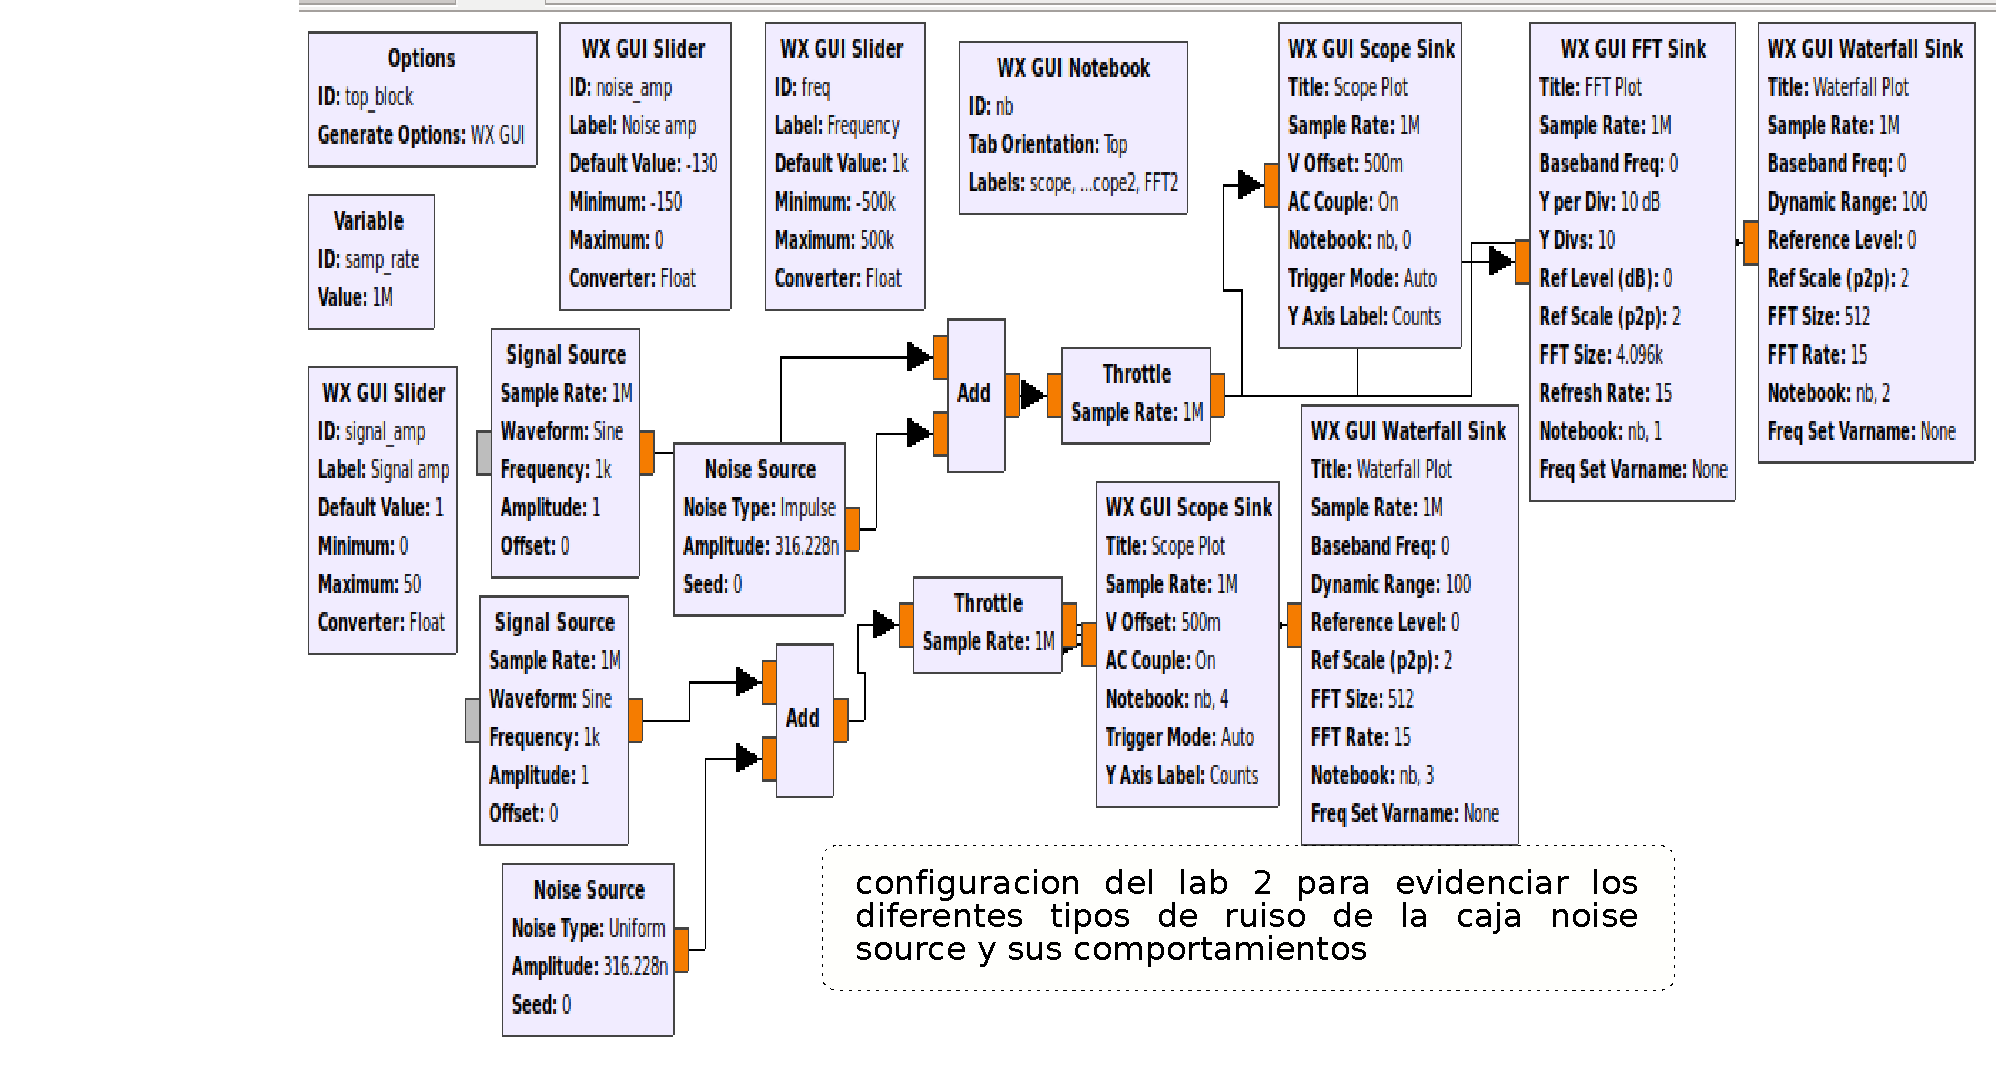
\includegraphics[width=\textwidth, height=0.58\textwidth]{soluciones/actividad-2-1/pdf/Rlab2_2.pdf}
\end{figure}
\end{frame}
%--------------------------------
\begin{frame}{Respuesta actividad 2 lab 2}
\begin{figure}[H]
\centering
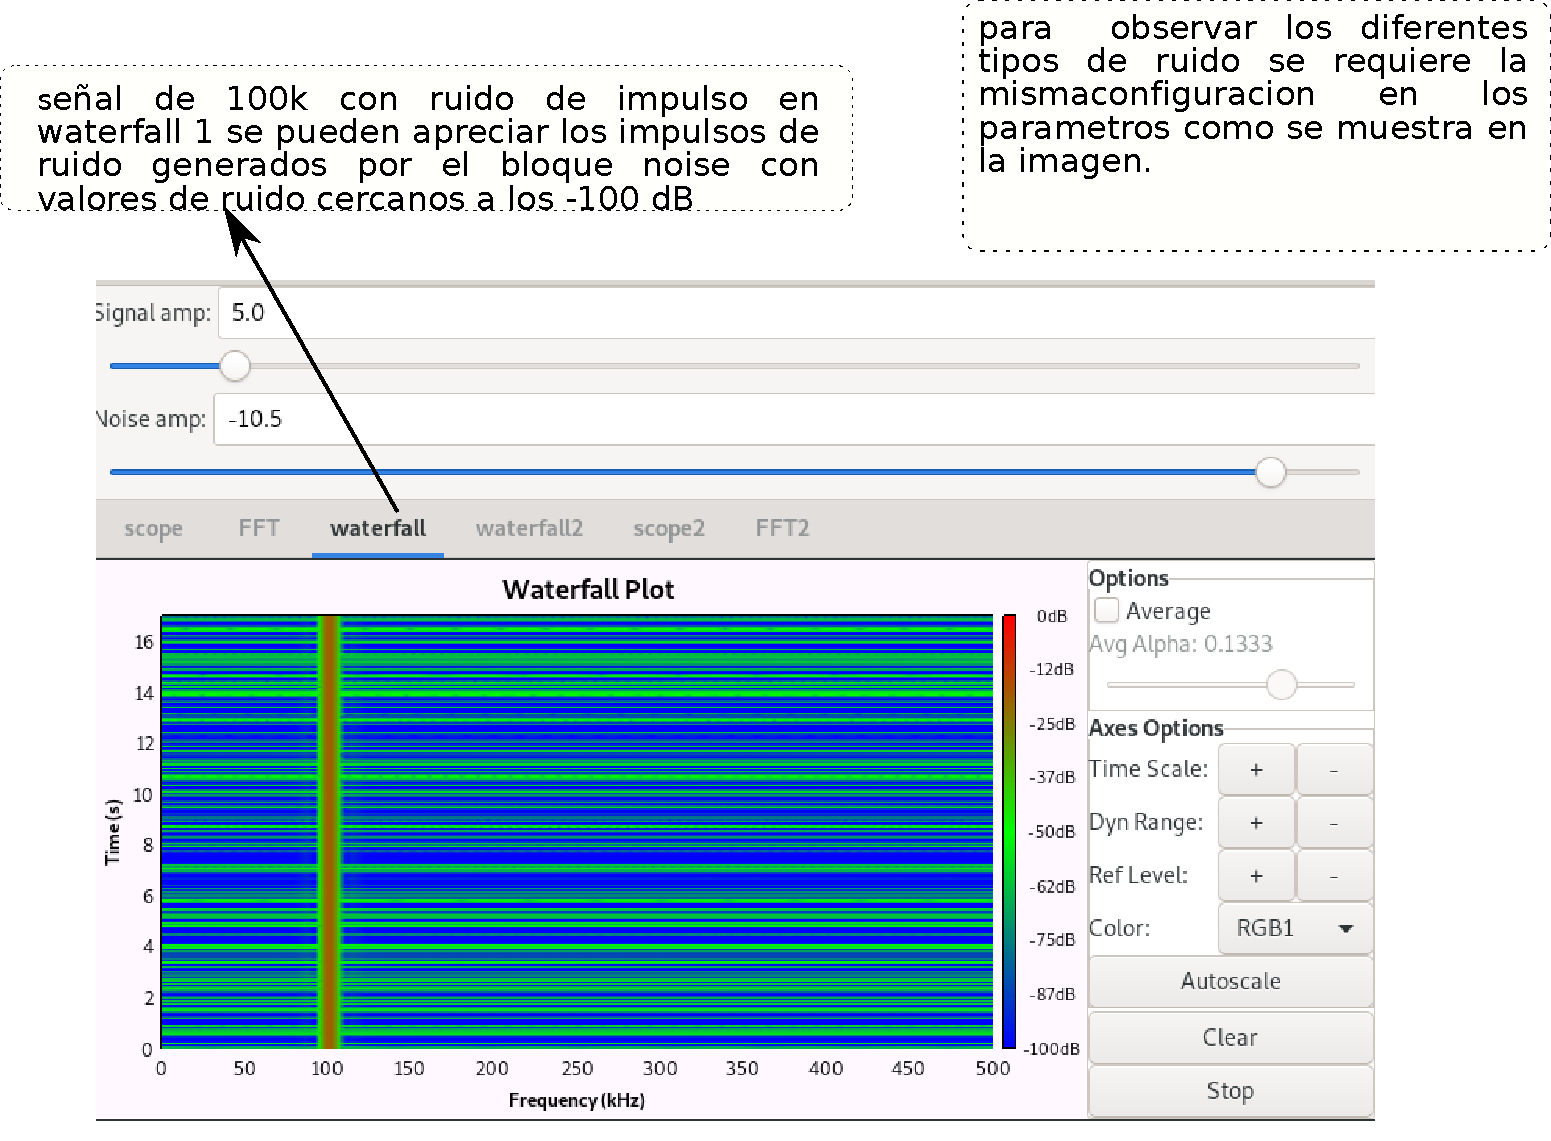
\includegraphics[width=\textwidth, height=0.58\textwidth]{soluciones/actividad-2-1/pdf/Rlab2_3.pdf}
\end{figure}
\end{frame}
%--------------------------------
\begin{frame}{Respuesta actividad 2 lab 2}
\begin{figure}[H]
\centering
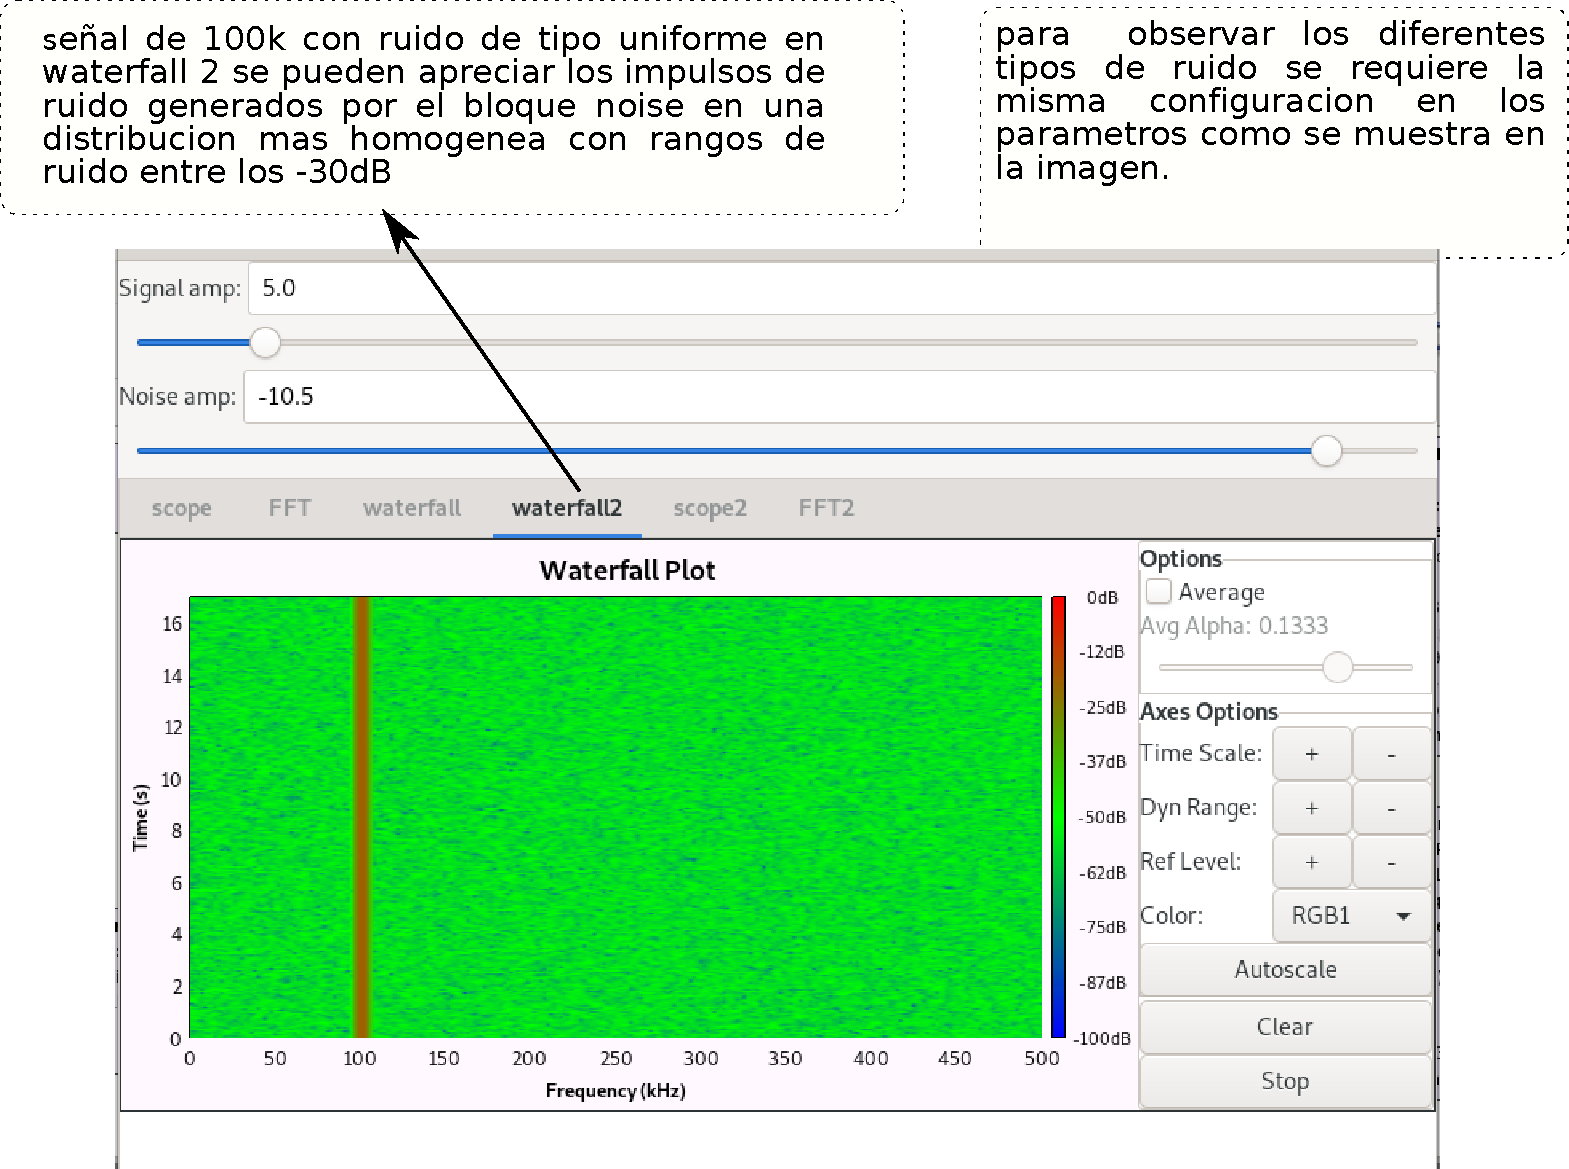
\includegraphics[width=\textwidth, height=0.58\textwidth]{soluciones/actividad-2-1/pdf/Rlab2_4.pdf}
\end{figure}
\end{frame}
%--------------------------------
\begin{frame}{Respuesta actividad 2 lab 2}
\begin{figure}[H]
\centering
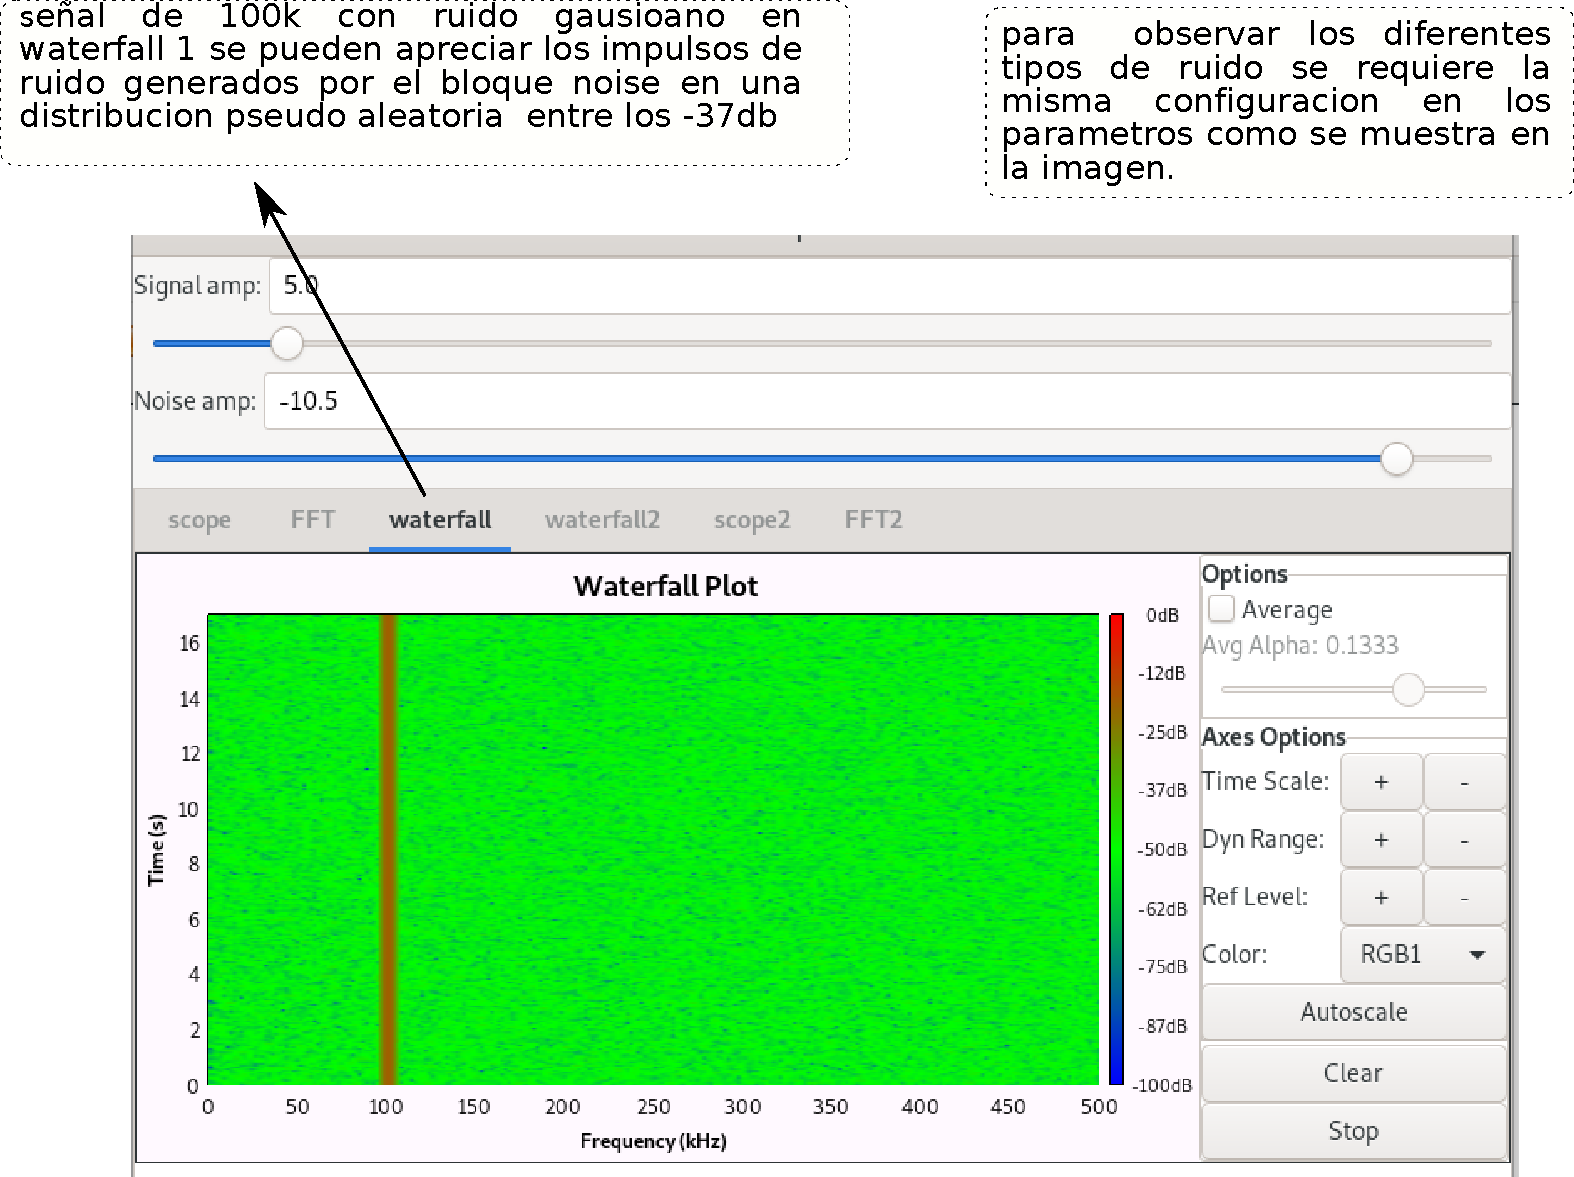
\includegraphics[width=\textwidth, height=0.58\textwidth]{soluciones/actividad-2-1/pdf/Rlab2_5.pdf}
\end{figure}
\end{frame}
%--------------------------------
\begin{frame}{Respuesta actividad 2 lab 2}
\begin{figure}[H]
\centering
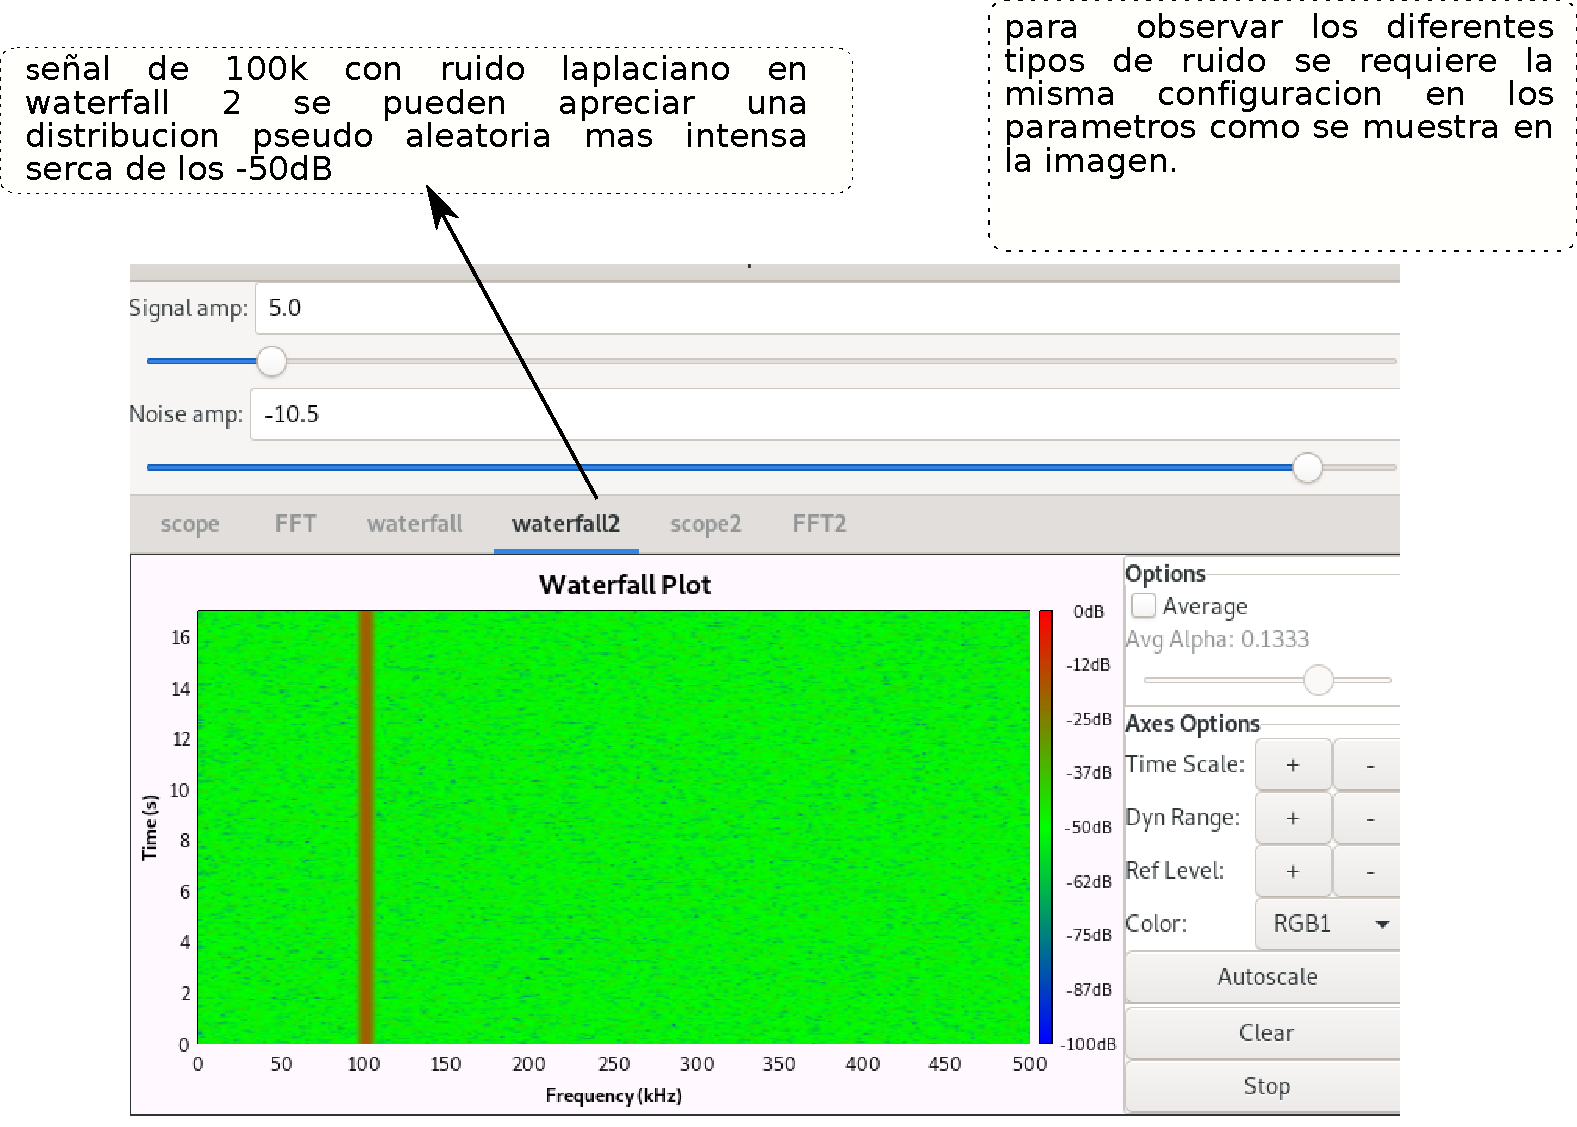
\includegraphics[width=\textwidth, height=0.58\textwidth]{soluciones/actividad-2-1/pdf/Rlab2_6.pdf}
\end{figure}
\end{frame}